\documentclass[letterpaper, reqno,11pt]{article}
\usepackage[margin=1.0in]{geometry}
\usepackage{color,latexsym,amsmath,amssymb,graphicx,float,listings,tikz}
\usepackage{hyperref}

\hypersetup{
colorlinks=true,
linkcolor=magenta,
filecolor=magenta,
urlcolor=cyan,
}

\lstset{
basicstyle=\ttfamily,
columns=fullflexible,
frame=single,
breaklines=true,
postbreak=\mbox{\textcolor{red}{$\hookrightarrow$}\space},
}

\graphicspath{ {images/} }

\begin{document}
\pagenumbering{arabic}
\title{PHYS408 Homework 2}
\date{13/02/24}
\author{Xander Naumenko}
\maketitle

{\medskip\noindent\bf Question 1a.} In class, we derived the following result in the Fraunhofer limit:
\[
    E(x',y')\approx \frac{e^{ikz}}{i\lambda z}e^{ik \frac{x'^2+y'^2}{2z}}\tilde E(k_x,k_y)
.\]
Thus all we have to do is compute the Fourier transform of the two slits. We can describe the slits as two shifted rectangles (assuming the input field $E$ is uniform and has magnitude 1):
\[
E(x,y) = \text{rect}\left(\frac{x}{d_x}\right)\left( \text{rect}\left( \frac{y-\Delta /2}{d_y} \right) +\text{rect}\left( \frac{y+\Delta /2}{d_y} \right)  \right) 
.\]
Also recall the following transform:
\[
    \mathcal F(\text{rect}(ax))=\frac{1}{|a|}\text{sinc}\left( \frac{k_x}{a} \right) 
.\]
Using this we get the following:
\[
    \tilde E(k_x, k_y) = d_xd_y \text{sinc}\left(\frac{d_xk_x}{2\pi}\right)\text{sinc}\left(\frac{d_yk_y}{2\pi}\right)\left( e^{i\Delta k_y /2}+e^{-i\Delta k_y /2} \right) 
.\]
Intensity is proportional to electric field squared, and since the question just asks for the distribution the constant factors can be discarded:
\[
I(x',y') \propto |E(x',y')|^2=\frac{1}{(\lambda z)^2} \text{sinc}^2\left(\frac{d_xk_x}{2\pi}\right)\text{sinc}^2\left(\frac{d_yk_y}{2\pi}\right)\sin^2\left( \frac{\Delta k_y}{2} \right) 
\]
where as usual $k_x= \frac{kx'}{z}$ and $k_y=\frac{ky'}{z}$.

{\medskip\noindent\bf Question 1b.} See figure \ref{fig:q1b}. The code used to produced the graphs is here:
\begin{lstlisting}
import numpy as np
import matplotlib.pyplot as plt

dx = 0.01
dy = 0.001
delta = 0.005
lam = 500e-9
z = 50

k = 2*np.pi/lam

x = np.linspace(-0.05, 0.05, 1000)
y = np.linspace(-0.05, 0.05, 1000)

kx = k*x/z
ky = k*y/z

Ix = (lam/z*np.sinc(dx*kx/(4*np.pi)))**2
Iy = (lam/z*np.sinc(dy*ky/(4*np.pi))*np.sin(delta*ky/2))**2

plt.plot(x, Ix)
plt.title("Intensity of Double Slit for y=0 Axis")
plt.xlabel("x' (m)")
plt.ylabel("I (W/m$^2$)")
plt.show()

plt.plot(y, Iy)
plt.title("Intensity of Double Slit for x=0 Axis")
plt.xlabel("y' (m)")
plt.ylabel("I (W/m$^2$)")

plt.show()
\end{lstlisting}

\begin{figure}[htpb]
    \centering
    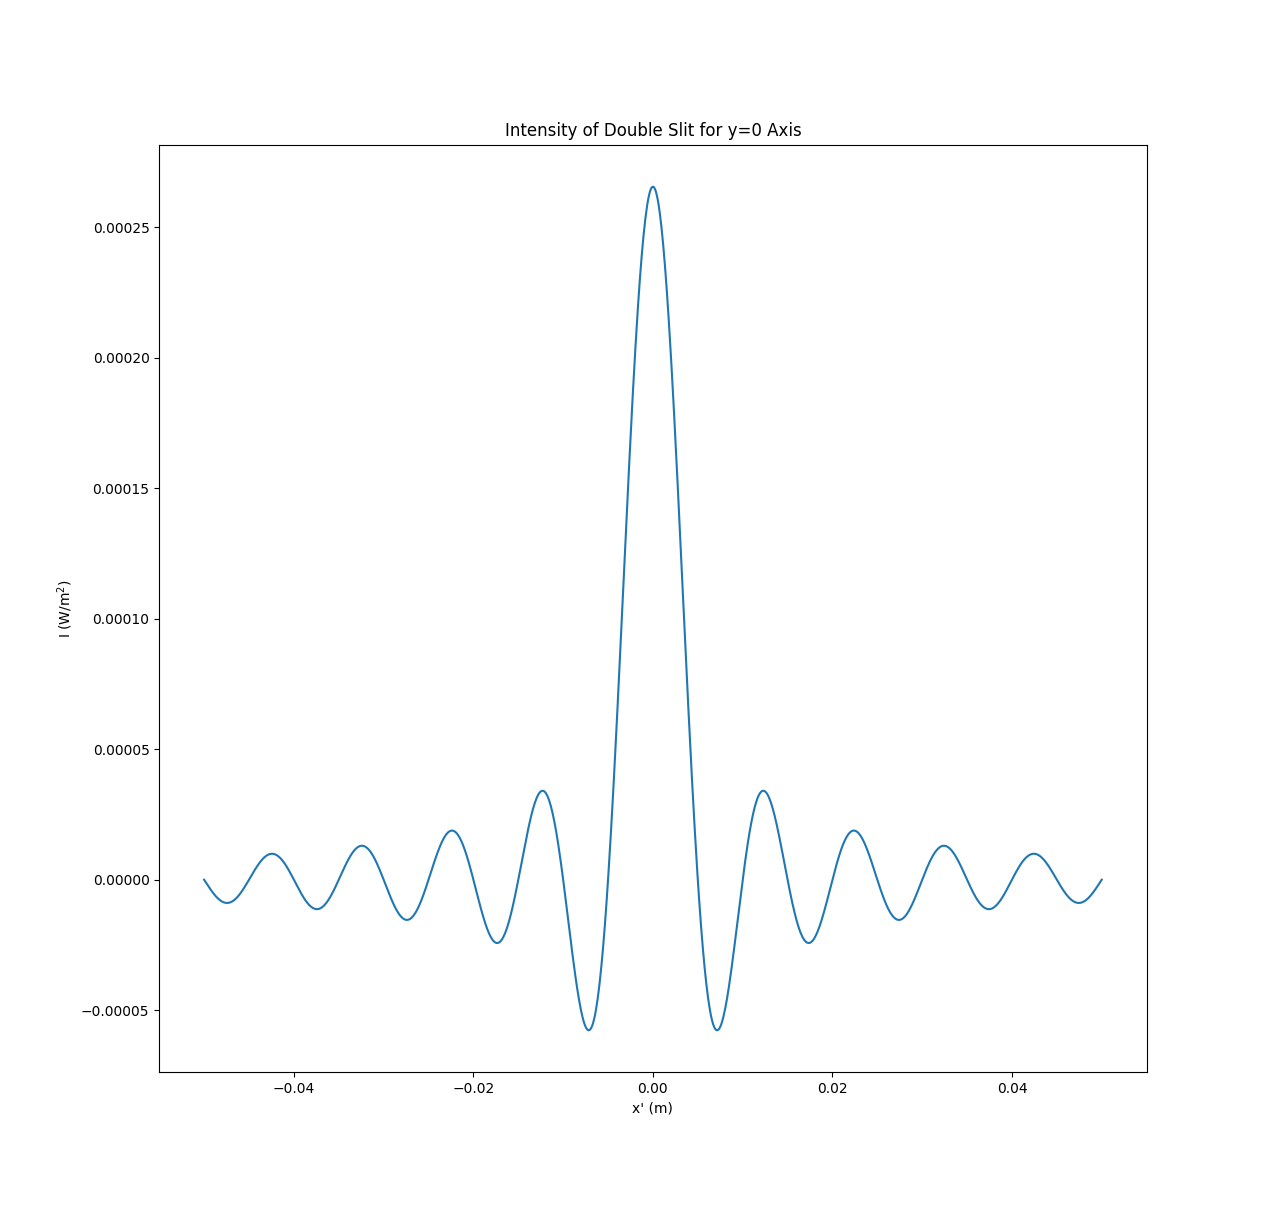
\includegraphics[width=0.6\textwidth]{q1x}
    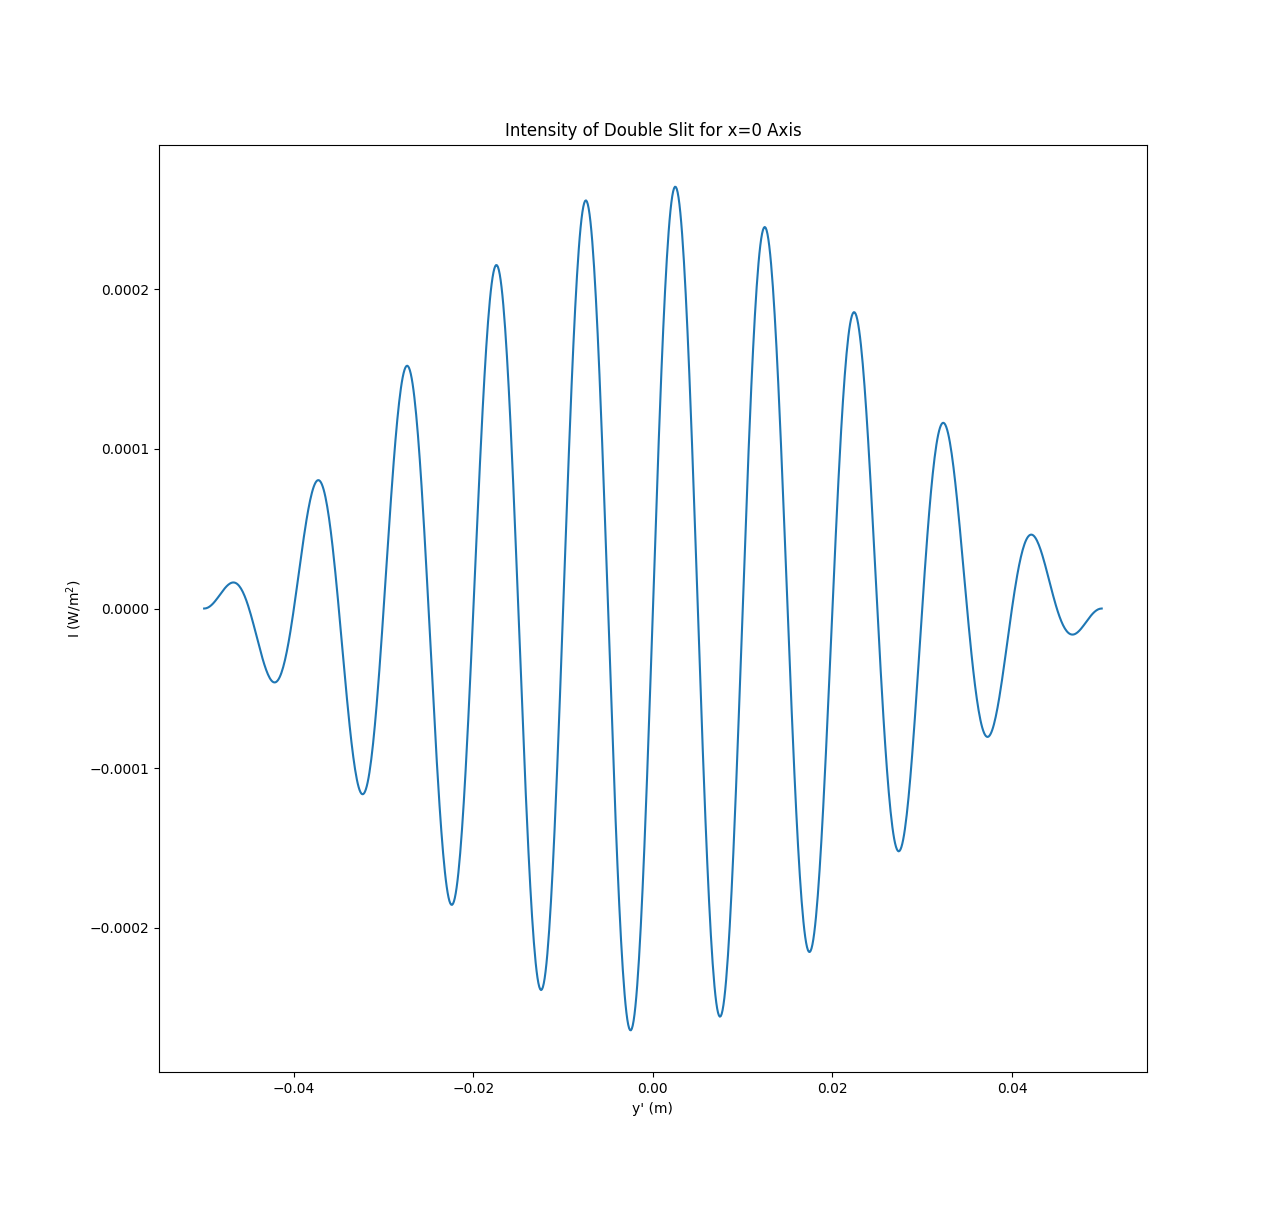
\includegraphics[width=0.6\textwidth]{q1y}
    \caption{Graphs for question 1b.}
    \label{fig:q1b}
\end{figure}

{\medskip\noindent\bf Question 1c.} The Fraunhofer limit applies only if $\frac{x^2}{\lambda}, \frac{y^2}{\lambda} \ll \frac{z}{\pi}$. In our case, these are $\frac{(d_x/2)^2}{\lambda}=50$ and $\frac{(d_y /2)^2}{\lambda}=\frac{1}{2}$. In comparison to $\frac{z}{\pi}\approx 15.9$, we see that the $x$-axis is no in the Fraunhofer approximation, so our results above are not totally valid.

{\medskip\noindent\bf Question 1d.} 


% {\medskip\noindent\bf Question 2a.} Width the addition of the finite length, the thickness function is 
% \[
%     d(x)=\left( \overline{d}+\frac{d_0}{2} \sin\left( 2\pi x /\Lambda \right)  \right)\text{rect}(x /d_x)
% .\]
% The Fourier transform of the left hand side is 

{\medskip\noindent\bf Question 2a.} The phase function is 



\end{document}
